\documentclass[10pt]{beamer}

\usepackage[utf8]{inputenc}
\usepackage[spanish]{babel} % Español
\usepackage{graphicx}
\usepackage{tabularx} % Tablas ajustables
\usepackage{booktabs}
\usepackage{bm}
\usepackage{mathtools}
\usepackage{utopia} % Fuente Utopia
\usepackage{caption}
\usepackage{natbib}
\usepackage{hyperref}

\usetheme{CambridgeUS}
\usefonttheme{professionalfonts}

% Colores
\definecolor{myNewColorA}{RGB}{139,0,0}
\definecolor{myNewColorB}{RGB}{139,0,0}
\definecolor{myNewColorC}{RGB}{139,0,0}
\setbeamercolor*{palette primary}{bg=myNewColorC}
\setbeamercolor*{palette secondary}{bg=myNewColorB, fg = white}
\setbeamercolor*{palette tertiary}{bg=myNewColorA, fg = white}
\setbeamercolor*{titlelike}{fg=myNewColorA}
\setbeamercolor*{title}{bg=myNewColorA, fg = white}
\setbeamercolor*{item}{fg=myNewColorA}
\setbeamercolor*{caption name}{fg=myNewColorA}

% Fuentes de portada
\setbeamerfont{title}{size=\large}
\setbeamerfont{subtitle}{size=\small}
\setbeamerfont{author}{size=\small}
\setbeamerfont{date}{size=\small}
\setbeamerfont{institute}{size=\small}

% Título y portada
\title{Datos: extracción, descripción y análisis}
\date[\textcolor{white}{\today}]{\today}

\begin{document}

% Portada
\frame{\titlepage}
%---------------------------------------------------------------------------
%---------------- SLIDE 1 ----------------

\begin{frame}{Fuente, Web Scraping y limpieza}
\begin{itemize}
  \item \textbf{Fuente de los datos.} Reporte de Medición de Pobreza Monetaria y Desigualdad (GEIH 2018, DANE). Contiene información de ingresos, estrato, edad, sexo y horas trabajadas, entre otras.
  \medskip
  \item \textbf{Web scraping.} Los datos públicos se obtuvieron desde 
  \href{https://ignaciomsarmiento.github.io/GEIH2018_sample/}{\texttt{ignaciomsarmiento.github.io/GEIH2018\_sample/}} 
  navegando las 10 páginas de \emph{chunks} (\texttt{pages/geih\_page\_\{1..10\}.html}) y extrayendo las tablas HTML.
  \medskip
  \item \textbf{Limpieza y preparación.} 
  \begin{itemize}
    \item Filtro: ocupados, $\ge$ 18 años, sin salarios nulos/cero; se excluye cuenta propia.
    \item Depuración de variables: se eliminan columnas con todo NA / constante y con $>$60\% de NA.
    \item Imputación: (i) categóricas por moda dentro de \textit{estrato}; (ii) numéricas con KNN ($k=5$).
    \item Tratamiento de colas en ingresos: recorte en el percentil 97.5.
  \end{itemize}
  \medskip
  \item \textbf{Muestra final.} 9{,}892 observaciones y 19 variables de interés.
\end{itemize}
\end{frame}

%===================== SLIDE 2 =====================
\begin{frame}{Estadística descriptiva}
\centering
\scriptsize
\textbf{(a) Variables numéricas} \par\medskip
\resizebox{\textwidth}{!}{%
\begin{tabular}{lccccc}
\toprule
Variable & N & Media & Desv. Est. & Min & Max \\
\midrule
Salario mensual                  & 9,892 & 1,610,063 & 1,537,099 & 20,000 & 7,892,292 \\
Salario por hora                 & 9,892 & 8,121.29  & 8,099.11  & 326.67 & 41,470.34 \\
ln(Salario)                      & 9,892 & 8.71      & 0.69      & 5.79   & 10.63 \\
Horas trabajadas                 & 9,892 & 48.34     & 12.25     & 1.00   & 130.00 \\
Edad                             & 9,892 & 36.24     & 12.02     & 18.00  & 86.00 \\
Mujer (1 = Sí)                   & 9,892 & 0.50      & 0.50      & 0.00   & 1.00 \\
Trabaja en microempresa (1 = Sí) & 9,892 & 0.23      & 0.42      & 0.00   & 1.00 \\
Trabajo formal (1 = Sí)          & 9,892 & 0.77      & 0.42      & 0.00   & 1.00 \\
\bottomrule
\end{tabular}
}
\medskip

\textbf{(b) Variables categóricas} \par\medskip
\resizebox{\textwidth}{!}{%
\begin{tabular}{lcccc}
\toprule
Variable & Categoría & Descripción & Frecuencia & Porcentaje \\
\midrule
Nivel educativo   & 7  & Educación terciaria              & 4,478 & 45.27\% \\
Oficio            & 39 & Apoyo administrativo y logístico &   814 & 8.23\% \\
Tamaño de empresa & 5  & $>$ 50 empleados                 & 5,107 & 51.63\% \\
Tipo de empleo    & 1  & Empleado de empresa particular   & 8,757 & 88.53\% \\
\bottomrule
\end{tabular}
}
\medskip

\raggedright\footnotesize\textit{Nota:} Panel (a) reporta N, media, desviación estándar, mínimo y máximo. Panel (b) reporta categoría modal, su descripción, frecuencia y porcentaje.
\end{frame}

%===================== SLIDE 3 =====================
\begin{frame}{Distribuciones del salario}

\scriptsize

\begin{itemize}
  \item Los salarios se concentran en la parte más baja de la distribución, entre los \$3{,}000 y los \$9{,}000 pesos por hora.
  \item Los salarios más altos siguen empujando las estadísticas hacia arriba, a pesar del corte de ingresos en el percentil 97.5. Se observa una cola con casi 500 individuos con ingresos mayores a \$40{,}000 por hora.
  \item Esto sugiere una importante desigualdad salarial en un contexto de brechas socioeconómicas pronunciadas como Bogotá.
\end{itemize}

\medskip

\begin{columns}[T,onlytextwidth]
  \column{0.5\textwidth}
  \centering
  \textbf{Salario por hora}\par\medskip
  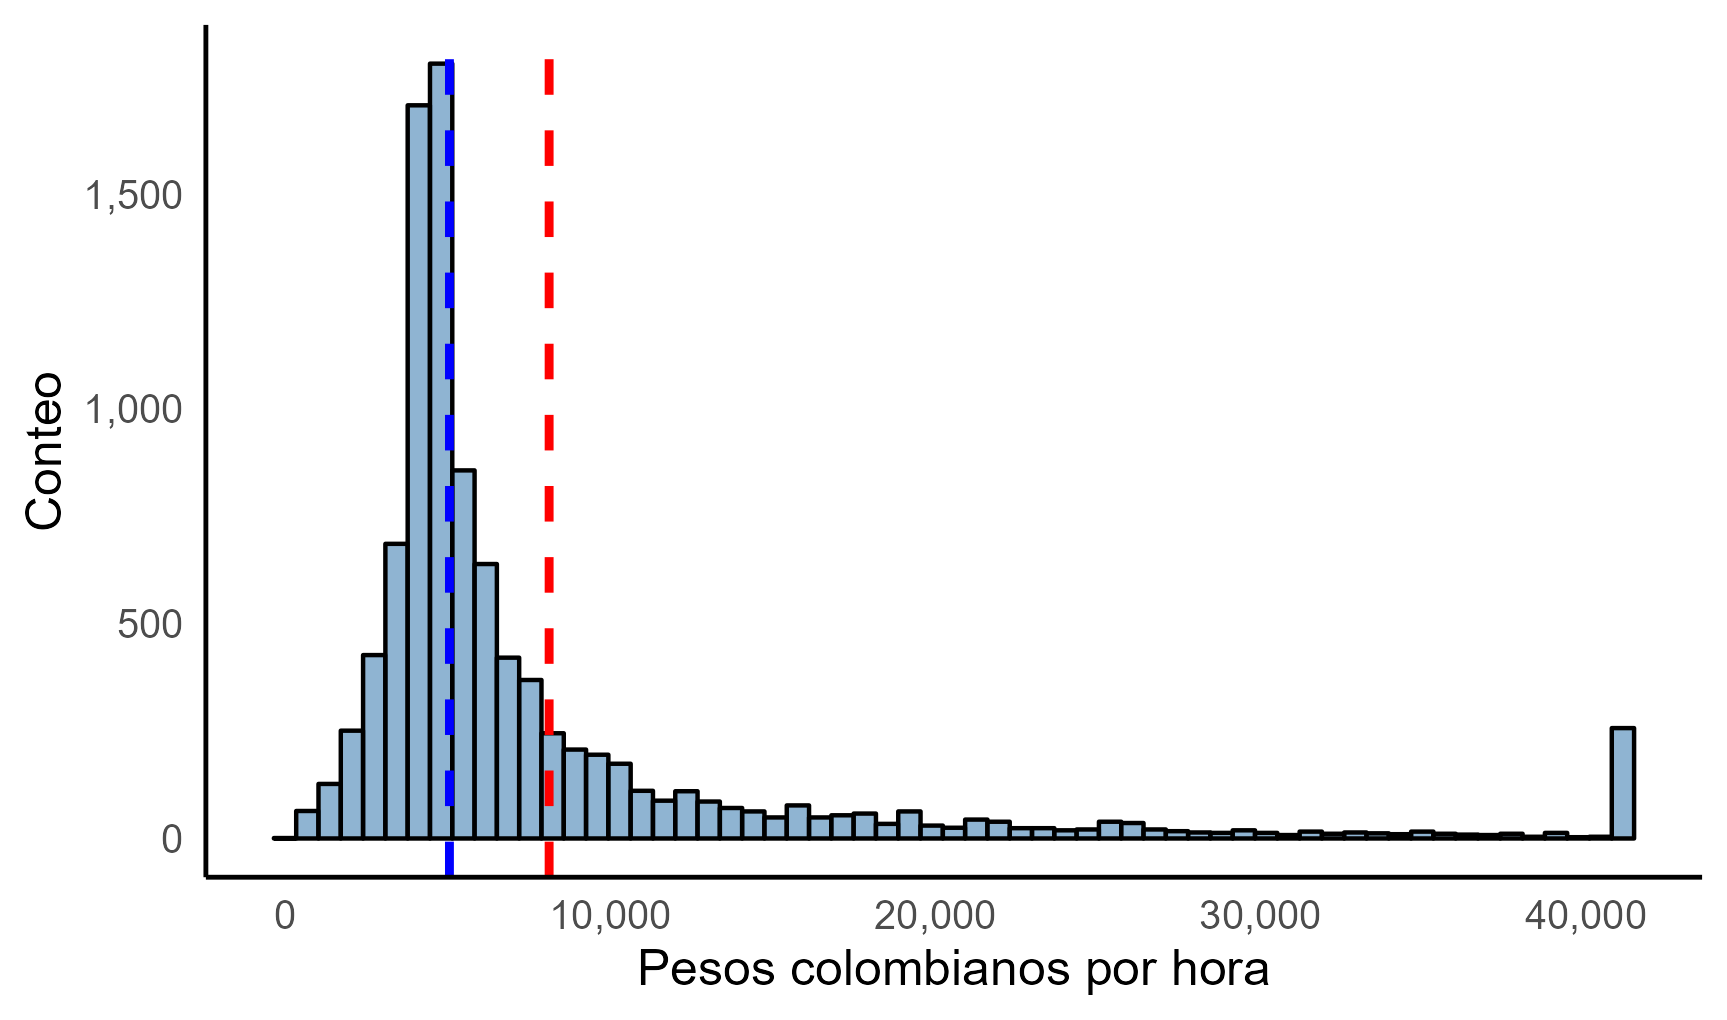
\includegraphics[width=\linewidth]{../../views/1_histo_sal.png}

  \column{0.5\textwidth}
  \centering
  \textbf{Logaritmo natural del salario}\par\medskip
  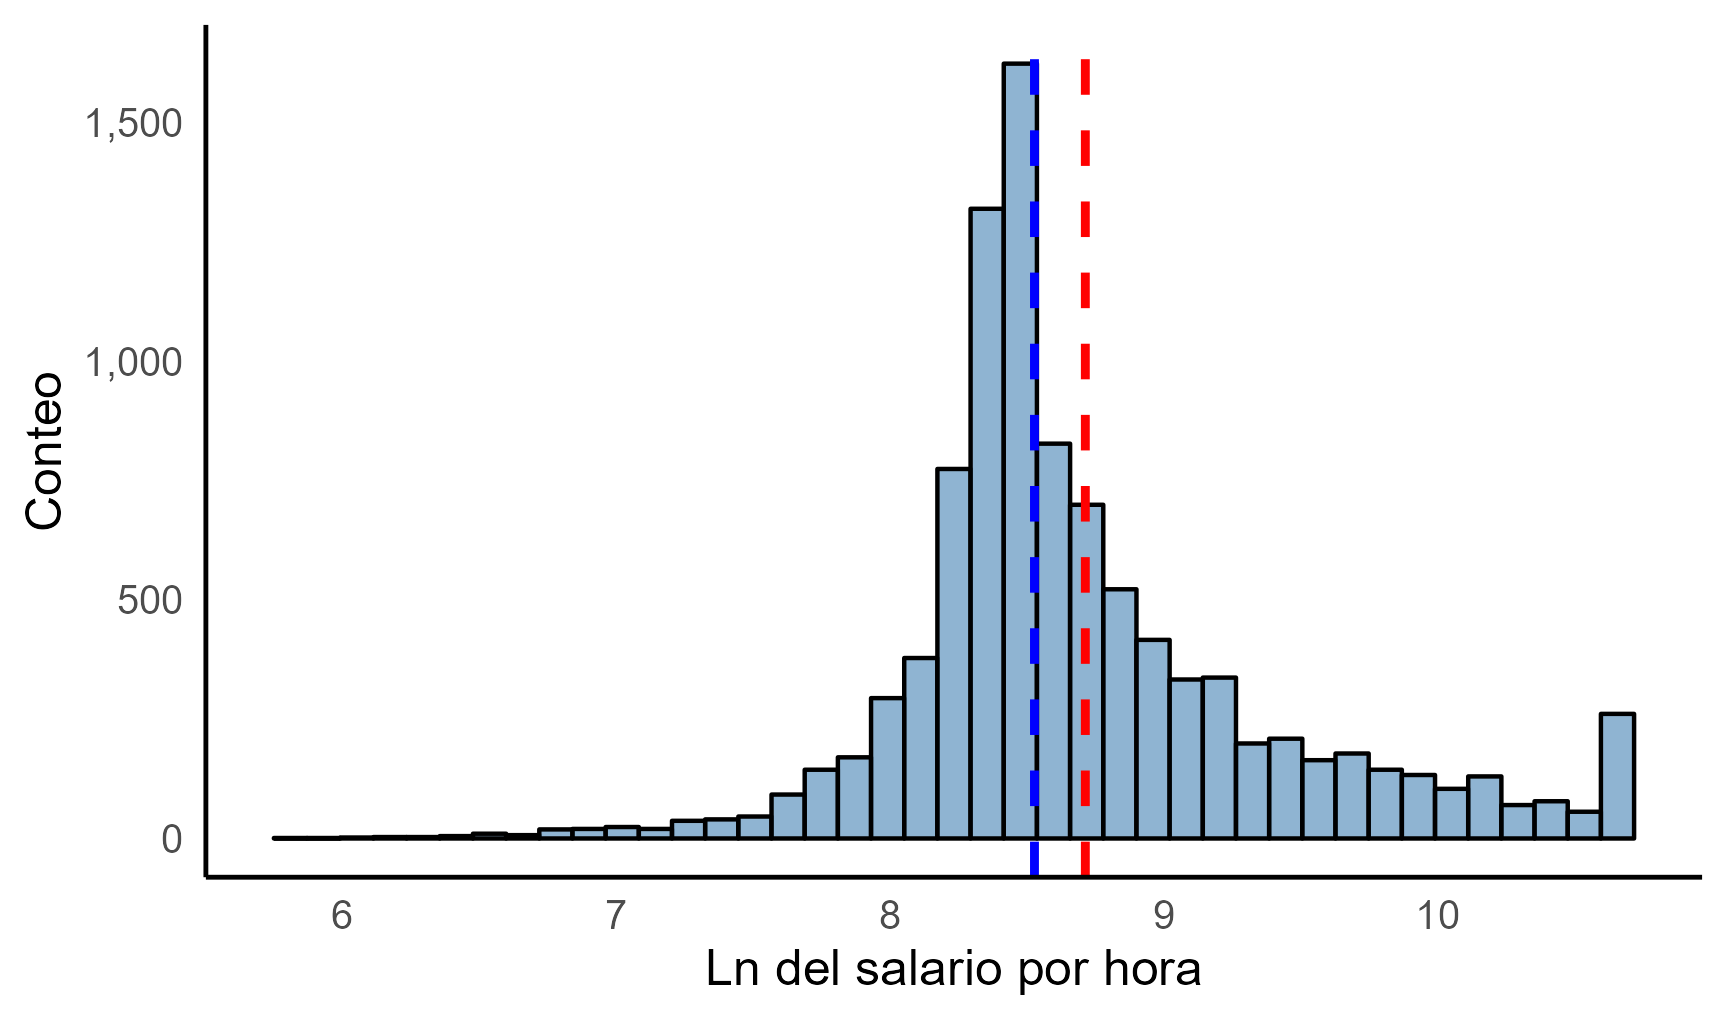
\includegraphics[width=\linewidth]{../../views/1_histo_sal_hora.png}
\end{columns}

\medskip
\footnotesize
\textit{Nota:} Histogramas con líneas verticales: roja = media, azul = mediana. Los salarios se concentran en la parte baja; el log-salario es más simétrico.
\end{frame}

%---------------------

\end{document}